% Options for packages loaded elsewhere
% Options for packages loaded elsewhere
\PassOptionsToPackage{unicode}{hyperref}
\PassOptionsToPackage{hyphens}{url}
\PassOptionsToPackage{dvipsnames,svgnames,x11names}{xcolor}
%
\documentclass[
  letterpaper,
  DIV=11,
  numbers=noendperiod]{scrartcl}
\usepackage{xcolor}
\usepackage{amsmath,amssymb}
\setcounter{secnumdepth}{-\maxdimen} % remove section numbering
\usepackage{iftex}
\ifPDFTeX
  \usepackage[T1]{fontenc}
  \usepackage[utf8]{inputenc}
  \usepackage{textcomp} % provide euro and other symbols
\else % if luatex or xetex
  \usepackage{unicode-math} % this also loads fontspec
  \defaultfontfeatures{Scale=MatchLowercase}
  \defaultfontfeatures[\rmfamily]{Ligatures=TeX,Scale=1}
\fi
\usepackage{lmodern}
\ifPDFTeX\else
  % xetex/luatex font selection
\fi
% Use upquote if available, for straight quotes in verbatim environments
\IfFileExists{upquote.sty}{\usepackage{upquote}}{}
\IfFileExists{microtype.sty}{% use microtype if available
  \usepackage[]{microtype}
  \UseMicrotypeSet[protrusion]{basicmath} % disable protrusion for tt fonts
}{}
\makeatletter
\@ifundefined{KOMAClassName}{% if non-KOMA class
  \IfFileExists{parskip.sty}{%
    \usepackage{parskip}
  }{% else
    \setlength{\parindent}{0pt}
    \setlength{\parskip}{6pt plus 2pt minus 1pt}}
}{% if KOMA class
  \KOMAoptions{parskip=half}}
\makeatother
% Make \paragraph and \subparagraph free-standing
\makeatletter
\ifx\paragraph\undefined\else
  \let\oldparagraph\paragraph
  \renewcommand{\paragraph}{
    \@ifstar
      \xxxParagraphStar
      \xxxParagraphNoStar
  }
  \newcommand{\xxxParagraphStar}[1]{\oldparagraph*{#1}\mbox{}}
  \newcommand{\xxxParagraphNoStar}[1]{\oldparagraph{#1}\mbox{}}
\fi
\ifx\subparagraph\undefined\else
  \let\oldsubparagraph\subparagraph
  \renewcommand{\subparagraph}{
    \@ifstar
      \xxxSubParagraphStar
      \xxxSubParagraphNoStar
  }
  \newcommand{\xxxSubParagraphStar}[1]{\oldsubparagraph*{#1}\mbox{}}
  \newcommand{\xxxSubParagraphNoStar}[1]{\oldsubparagraph{#1}\mbox{}}
\fi
\makeatother

\usepackage{color}
\usepackage{fancyvrb}
\newcommand{\VerbBar}{|}
\newcommand{\VERB}{\Verb[commandchars=\\\{\}]}
\DefineVerbatimEnvironment{Highlighting}{Verbatim}{commandchars=\\\{\}}
% Add ',fontsize=\small' for more characters per line
\usepackage{framed}
\definecolor{shadecolor}{RGB}{241,243,245}
\newenvironment{Shaded}{\begin{snugshade}}{\end{snugshade}}
\newcommand{\AlertTok}[1]{\textcolor[rgb]{0.68,0.00,0.00}{#1}}
\newcommand{\AnnotationTok}[1]{\textcolor[rgb]{0.37,0.37,0.37}{#1}}
\newcommand{\AttributeTok}[1]{\textcolor[rgb]{0.40,0.45,0.13}{#1}}
\newcommand{\BaseNTok}[1]{\textcolor[rgb]{0.68,0.00,0.00}{#1}}
\newcommand{\BuiltInTok}[1]{\textcolor[rgb]{0.00,0.23,0.31}{#1}}
\newcommand{\CharTok}[1]{\textcolor[rgb]{0.13,0.47,0.30}{#1}}
\newcommand{\CommentTok}[1]{\textcolor[rgb]{0.37,0.37,0.37}{#1}}
\newcommand{\CommentVarTok}[1]{\textcolor[rgb]{0.37,0.37,0.37}{\textit{#1}}}
\newcommand{\ConstantTok}[1]{\textcolor[rgb]{0.56,0.35,0.01}{#1}}
\newcommand{\ControlFlowTok}[1]{\textcolor[rgb]{0.00,0.23,0.31}{\textbf{#1}}}
\newcommand{\DataTypeTok}[1]{\textcolor[rgb]{0.68,0.00,0.00}{#1}}
\newcommand{\DecValTok}[1]{\textcolor[rgb]{0.68,0.00,0.00}{#1}}
\newcommand{\DocumentationTok}[1]{\textcolor[rgb]{0.37,0.37,0.37}{\textit{#1}}}
\newcommand{\ErrorTok}[1]{\textcolor[rgb]{0.68,0.00,0.00}{#1}}
\newcommand{\ExtensionTok}[1]{\textcolor[rgb]{0.00,0.23,0.31}{#1}}
\newcommand{\FloatTok}[1]{\textcolor[rgb]{0.68,0.00,0.00}{#1}}
\newcommand{\FunctionTok}[1]{\textcolor[rgb]{0.28,0.35,0.67}{#1}}
\newcommand{\ImportTok}[1]{\textcolor[rgb]{0.00,0.46,0.62}{#1}}
\newcommand{\InformationTok}[1]{\textcolor[rgb]{0.37,0.37,0.37}{#1}}
\newcommand{\KeywordTok}[1]{\textcolor[rgb]{0.00,0.23,0.31}{\textbf{#1}}}
\newcommand{\NormalTok}[1]{\textcolor[rgb]{0.00,0.23,0.31}{#1}}
\newcommand{\OperatorTok}[1]{\textcolor[rgb]{0.37,0.37,0.37}{#1}}
\newcommand{\OtherTok}[1]{\textcolor[rgb]{0.00,0.23,0.31}{#1}}
\newcommand{\PreprocessorTok}[1]{\textcolor[rgb]{0.68,0.00,0.00}{#1}}
\newcommand{\RegionMarkerTok}[1]{\textcolor[rgb]{0.00,0.23,0.31}{#1}}
\newcommand{\SpecialCharTok}[1]{\textcolor[rgb]{0.37,0.37,0.37}{#1}}
\newcommand{\SpecialStringTok}[1]{\textcolor[rgb]{0.13,0.47,0.30}{#1}}
\newcommand{\StringTok}[1]{\textcolor[rgb]{0.13,0.47,0.30}{#1}}
\newcommand{\VariableTok}[1]{\textcolor[rgb]{0.07,0.07,0.07}{#1}}
\newcommand{\VerbatimStringTok}[1]{\textcolor[rgb]{0.13,0.47,0.30}{#1}}
\newcommand{\WarningTok}[1]{\textcolor[rgb]{0.37,0.37,0.37}{\textit{#1}}}

\usepackage{longtable,booktabs,array}
\usepackage{calc} % for calculating minipage widths
% Correct order of tables after \paragraph or \subparagraph
\usepackage{etoolbox}
\makeatletter
\patchcmd\longtable{\par}{\if@noskipsec\mbox{}\fi\par}{}{}
\makeatother
% Allow footnotes in longtable head/foot
\IfFileExists{footnotehyper.sty}{\usepackage{footnotehyper}}{\usepackage{footnote}}
\makesavenoteenv{longtable}
\usepackage{graphicx}
\makeatletter
\newsavebox\pandoc@box
\newcommand*\pandocbounded[1]{% scales image to fit in text height/width
  \sbox\pandoc@box{#1}%
  \Gscale@div\@tempa{\textheight}{\dimexpr\ht\pandoc@box+\dp\pandoc@box\relax}%
  \Gscale@div\@tempb{\linewidth}{\wd\pandoc@box}%
  \ifdim\@tempb\p@<\@tempa\p@\let\@tempa\@tempb\fi% select the smaller of both
  \ifdim\@tempa\p@<\p@\scalebox{\@tempa}{\usebox\pandoc@box}%
  \else\usebox{\pandoc@box}%
  \fi%
}
% Set default figure placement to htbp
\def\fps@figure{htbp}
\makeatother





\setlength{\emergencystretch}{3em} % prevent overfull lines

\providecommand{\tightlist}{%
  \setlength{\itemsep}{0pt}\setlength{\parskip}{0pt}}



 


\KOMAoption{captions}{tableheading}
\makeatletter
\@ifpackageloaded{caption}{}{\usepackage{caption}}
\AtBeginDocument{%
\ifdefined\contentsname
  \renewcommand*\contentsname{Table of contents}
\else
  \newcommand\contentsname{Table of contents}
\fi
\ifdefined\listfigurename
  \renewcommand*\listfigurename{List of Figures}
\else
  \newcommand\listfigurename{List of Figures}
\fi
\ifdefined\listtablename
  \renewcommand*\listtablename{List of Tables}
\else
  \newcommand\listtablename{List of Tables}
\fi
\ifdefined\figurename
  \renewcommand*\figurename{Figure}
\else
  \newcommand\figurename{Figure}
\fi
\ifdefined\tablename
  \renewcommand*\tablename{Table}
\else
  \newcommand\tablename{Table}
\fi
}
\@ifpackageloaded{float}{}{\usepackage{float}}
\floatstyle{ruled}
\@ifundefined{c@chapter}{\newfloat{codelisting}{h}{lop}}{\newfloat{codelisting}{h}{lop}[chapter]}
\floatname{codelisting}{Listing}
\newcommand*\listoflistings{\listof{codelisting}{List of Listings}}
\makeatother
\makeatletter
\makeatother
\makeatletter
\@ifpackageloaded{caption}{}{\usepackage{caption}}
\@ifpackageloaded{subcaption}{}{\usepackage{subcaption}}
\makeatother
\usepackage{bookmark}
\IfFileExists{xurl.sty}{\usepackage{xurl}}{} % add URL line breaks if available
\urlstyle{same}
\hypersetup{
  pdftitle={Data visualization with R: reporting with Quarto},
  pdfauthor={Andrea Cappozzo},
  colorlinks=true,
  linkcolor={blue},
  filecolor={Maroon},
  citecolor={Blue},
  urlcolor={Blue},
  pdfcreator={LaTeX via pandoc}}


\title{Data visualization with R: reporting with Quarto}
\usepackage{etoolbox}
\makeatletter
\providecommand{\subtitle}[1]{% add subtitle to \maketitle
  \apptocmd{\@title}{\par {\large #1 \par}}{}{}
}
\makeatother
\subtitle{Master in Data science for Management AY 2025/2026}
\author{Andrea Cappozzo}
\date{}
\begin{document}
\maketitle


\subsection{Meet Quarto}\label{meet-quarto}

Quarto is an \textbf{open-source scientific and technical publishing
system} that allows users to create dynamic documents, presentations,
blogs, and websites using plain text files (.qmd). It supports multiple
programming languages (like \emph{R, Python, and Julia}) and integrates
with Markdown to generate high-quality, reproducible reports in various
formats, including HTML, PDF, and Word. To learn more about Quarto, see
\url{https://quarto.org}. Disclaimer: the following section is an
adaptation of the
\href{https://quarto.org/docs/get-started/hello/rstudio.html}{Tutorial:
Hello, Quarto} that can be found in the Quarto website.

\subsection{An end-to-end example: meet the
penguins!}\label{an-end-to-end-example-meet-the-penguins}

The \texttt{penguins} data from the
\href{https://allisonhorst.github.io/palmerpenguins}{palmerpenguins}
package contains size measurements for 344 penguins from three species
observed on three islands in the Palmer Archipelago, Antarctica.

\pandocbounded{
\includegraphics[keepaspectratio]{lter_penguins.png}}

The plot below shows the relationship between flipper and bill lengths
of these penguins.

\begin{Shaded}
\begin{Highlighting}[]
\FunctionTok{ggplot}\NormalTok{(penguins, }\FunctionTok{aes}\NormalTok{(}\AttributeTok{x =}\NormalTok{ flipper\_length\_mm, }\AttributeTok{y =}\NormalTok{ bill\_length\_mm)) }\SpecialCharTok{+}
  \FunctionTok{geom\_point}\NormalTok{(}\FunctionTok{aes}\NormalTok{(}\AttributeTok{color =}\NormalTok{ species, }\AttributeTok{shape =}\NormalTok{ species)) }\SpecialCharTok{+}
  \FunctionTok{scale\_color\_manual}\NormalTok{(}\AttributeTok{values =} \FunctionTok{c}\NormalTok{(}\StringTok{"darkorange"}\NormalTok{, }\StringTok{"purple"}\NormalTok{, }\StringTok{"cyan4"}\NormalTok{)) }\SpecialCharTok{+}
  \FunctionTok{labs}\NormalTok{(}
    \AttributeTok{title =} \StringTok{"Flipper and bill length"}\NormalTok{,}
    \AttributeTok{subtitle =} \StringTok{"Dimensions for penguins at Palmer Station LTER"}\NormalTok{,}
    \AttributeTok{x =} \StringTok{"Flipper length (mm)"}\NormalTok{,}
    \AttributeTok{y =} \StringTok{"Bill length (mm)"}\NormalTok{,}
    \AttributeTok{color =} \StringTok{"Penguin species"}\NormalTok{,}
    \AttributeTok{shape =} \StringTok{"Penguin species"}
\NormalTok{  ) }\SpecialCharTok{+}
  \FunctionTok{theme\_minimal}\NormalTok{()}
\end{Highlighting}
\end{Shaded}

\pandocbounded{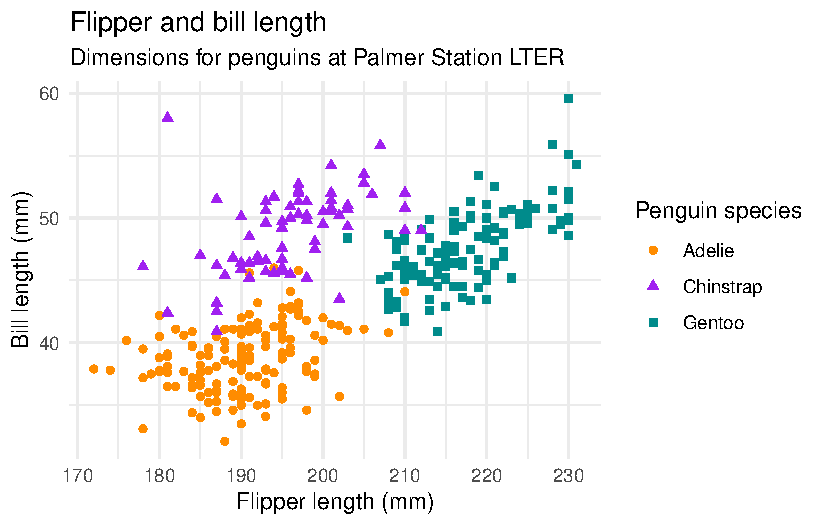
\includegraphics[keepaspectratio]{03-RDATAVIZ_26_quarto_files/figure-pdf/plot-penguins-1.pdf}}

First off, let us report some summary statistics of the dataset at hand

\begin{Shaded}
\begin{Highlighting}[]
\NormalTok{skimr}\SpecialCharTok{::}\FunctionTok{skim\_without\_charts}\NormalTok{(penguins)}
\end{Highlighting}
\end{Shaded}

\begin{longtable}[]{@{}ll@{}}
\caption{Data summary}\tabularnewline
\toprule\noalign{}
\endfirsthead
\endhead
\bottomrule\noalign{}
\endlastfoot
Name & penguins \\
Number of rows & 344 \\
Number of columns & 8 \\
\_\_\_\_\_\_\_\_\_\_\_\_\_\_\_\_\_\_\_\_\_\_\_ & \\
Column type frequency: & \\
factor & 3 \\
numeric & 5 \\
\_\_\_\_\_\_\_\_\_\_\_\_\_\_\_\_\_\_\_\_\_\_\_\_ & \\
Group variables & None \\
\end{longtable}

\textbf{Variable type: factor}

\begin{longtable}[]{@{}
  >{\raggedright\arraybackslash}p{(\linewidth - 10\tabcolsep) * \real{0.1687}}
  >{\raggedleft\arraybackslash}p{(\linewidth - 10\tabcolsep) * \real{0.1205}}
  >{\raggedleft\arraybackslash}p{(\linewidth - 10\tabcolsep) * \real{0.1687}}
  >{\raggedright\arraybackslash}p{(\linewidth - 10\tabcolsep) * \real{0.0964}}
  >{\raggedleft\arraybackslash}p{(\linewidth - 10\tabcolsep) * \real{0.1084}}
  >{\raggedright\arraybackslash}p{(\linewidth - 10\tabcolsep) * \real{0.3373}}@{}}
\toprule\noalign{}
\begin{minipage}[b]{\linewidth}\raggedright
skim\_variable
\end{minipage} & \begin{minipage}[b]{\linewidth}\raggedleft
n\_missing
\end{minipage} & \begin{minipage}[b]{\linewidth}\raggedleft
complete\_rate
\end{minipage} & \begin{minipage}[b]{\linewidth}\raggedright
ordered
\end{minipage} & \begin{minipage}[b]{\linewidth}\raggedleft
n\_unique
\end{minipage} & \begin{minipage}[b]{\linewidth}\raggedright
top\_counts
\end{minipage} \\
\midrule\noalign{}
\endhead
\bottomrule\noalign{}
\endlastfoot
species & 0 & 1.00 & FALSE & 3 & Ade: 152, Gen: 124, Chi: 68 \\
island & 0 & 1.00 & FALSE & 3 & Bis: 168, Dre: 124, Tor: 52 \\
sex & 11 & 0.97 & FALSE & 2 & mal: 168, fem: 165 \\
\end{longtable}

\textbf{Variable type: numeric}

\begin{longtable}[]{@{}
  >{\raggedright\arraybackslash}p{(\linewidth - 18\tabcolsep) * \real{0.1915}}
  >{\raggedleft\arraybackslash}p{(\linewidth - 18\tabcolsep) * \real{0.1064}}
  >{\raggedleft\arraybackslash}p{(\linewidth - 18\tabcolsep) * \real{0.1489}}
  >{\raggedleft\arraybackslash}p{(\linewidth - 18\tabcolsep) * \real{0.0851}}
  >{\raggedleft\arraybackslash}p{(\linewidth - 18\tabcolsep) * \real{0.0745}}
  >{\raggedleft\arraybackslash}p{(\linewidth - 18\tabcolsep) * \real{0.0745}}
  >{\raggedleft\arraybackslash}p{(\linewidth - 18\tabcolsep) * \real{0.0851}}
  >{\raggedleft\arraybackslash}p{(\linewidth - 18\tabcolsep) * \real{0.0851}}
  >{\raggedleft\arraybackslash}p{(\linewidth - 18\tabcolsep) * \real{0.0745}}
  >{\raggedleft\arraybackslash}p{(\linewidth - 18\tabcolsep) * \real{0.0745}}@{}}
\toprule\noalign{}
\begin{minipage}[b]{\linewidth}\raggedright
skim\_variable
\end{minipage} & \begin{minipage}[b]{\linewidth}\raggedleft
n\_missing
\end{minipage} & \begin{minipage}[b]{\linewidth}\raggedleft
complete\_rate
\end{minipage} & \begin{minipage}[b]{\linewidth}\raggedleft
mean
\end{minipage} & \begin{minipage}[b]{\linewidth}\raggedleft
sd
\end{minipage} & \begin{minipage}[b]{\linewidth}\raggedleft
p0
\end{minipage} & \begin{minipage}[b]{\linewidth}\raggedleft
p25
\end{minipage} & \begin{minipage}[b]{\linewidth}\raggedleft
p50
\end{minipage} & \begin{minipage}[b]{\linewidth}\raggedleft
p75
\end{minipage} & \begin{minipage}[b]{\linewidth}\raggedleft
p100
\end{minipage} \\
\midrule\noalign{}
\endhead
\bottomrule\noalign{}
\endlastfoot
bill\_length\_mm & 2 & 0.99 & 43.92 & 5.46 & 32.1 & 39.23 & 44.45 & 48.5
& 59.6 \\
bill\_depth\_mm & 2 & 0.99 & 17.15 & 1.97 & 13.1 & 15.60 & 17.30 & 18.7
& 21.5 \\
flipper\_length\_mm & 2 & 0.99 & 200.92 & 14.06 & 172.0 & 190.00 &
197.00 & 213.0 & 231.0 \\
body\_mass\_g & 2 & 0.99 & 4201.75 & 801.95 & 2700.0 & 3550.00 & 4050.00
& 4750.0 & 6300.0 \\
year & 0 & 1.00 & 2008.03 & 0.82 & 2007.0 & 2007.00 & 2008.00 & 2009.0 &
2009.0 \\
\end{longtable}

Given that we are in the process of becoming data scientists, we will

\begin{enumerate}
\def\labelenumi{\arabic{enumi}.}
\tightlist
\item
  build a simple linear regression model to regress \emph{Bill length}
  as a function of \emph{Flipper length}
\item
  compute coefficients and display the results
\item
  report everything in a self-contained format (including code, tables
  etc) using Quarto!
\end{enumerate}

In details, we are interested in estimating the coefficients \(\alpha\)
and \(\beta_{1}\) of the following statistical model:

\[
\operatorname{bill\_length\_mm} = \alpha + \beta_{1}(\operatorname{flipper\_length\_mm}) + \epsilon
\]

All the details of the statistical procedure will be thoroughly
explained in the Statistical Learning module, where you will explore the
general formulation:

\[
y=\alpha + \beta_1 x + \epsilon
\]

in which \(y\) is called the response variable and \(x\) the independent
variable. For now, the key point to understand is that we aim to examine
how the response variable, \(\operatorname{bill\_length\_mm}\), relates
to the independent variable, \(\operatorname{flipper\_length\_mm}\).

In R, this can be accomplished with the following line of code:

\begin{Shaded}
\begin{Highlighting}[]
\NormalTok{fit\_lm }\OtherTok{\textless{}{-}} \FunctionTok{lm}\NormalTok{(bill\_length\_mm }\SpecialCharTok{\textasciitilde{}}\NormalTok{ flipper\_length\_mm, }\AttributeTok{data =}\NormalTok{ penguins)}
\end{Highlighting}
\end{Shaded}

The \texttt{fit\_lm} object is a list with class lm that stands for
linear model. While again all the details regarding this type of model
will become clear soon enough, we can exploit the Quarto capabilities to
report results from the \texttt{fit\_lm} object. Specifically, we can
report a table summarizing the model coefficients using the
\texttt{kable} function, that allows for creating tables in LaTeX, HTML
and more.

\begin{Shaded}
\begin{Highlighting}[]
\FunctionTok{library}\NormalTok{(broom)}
\FunctionTok{library}\NormalTok{(knitr)}
\NormalTok{tab\_coef }\OtherTok{\textless{}{-}} \FunctionTok{tidy}\NormalTok{(fit\_lm)}
\NormalTok{tab\_coef}
\end{Highlighting}
\end{Shaded}

\begin{verbatim}
# A tibble: 2 x 5
  term              estimate std.error statistic  p.value
  <chr>                <dbl>     <dbl>     <dbl>    <dbl>
1 (Intercept)         -7.26     3.20       -2.27 2.38e- 2
2 flipper_length_mm    0.255    0.0159     16.0  1.74e-43
\end{verbatim}

\begin{Shaded}
\begin{Highlighting}[]
\NormalTok{tab\_coef}\SpecialCharTok{$}\NormalTok{p.value }\OtherTok{\textless{}{-}} \FunctionTok{formatC}\NormalTok{(tab\_coef}\SpecialCharTok{$}\NormalTok{p.value, }\AttributeTok{format =} \StringTok{"e"}\NormalTok{, }\AttributeTok{digits =} \DecValTok{2}\NormalTok{)}

\FunctionTok{kable}\NormalTok{(tab\_coef, }\AttributeTok{digits =} \DecValTok{3}\NormalTok{)}
\end{Highlighting}
\end{Shaded}

\begin{longtable}[]{@{}lrrrl@{}}
\toprule\noalign{}
term & estimate & std.error & statistic & p.value \\
\midrule\noalign{}
\endhead
\bottomrule\noalign{}
\endlastfoot
(Intercept) & -7.265 & 3.200 & -2.270 & 2.38e-02 \\
flipper\_length\_mm & 0.255 & 0.016 & 16.034 & 1.74e-43 \\
\end{longtable}

Look at the difference of having or not used \texttt{kable} in the
previous call. In a report, generally we tend to include the least
amount of code as possible: for example if we only want to report the
table wihout include the code used to generate it we can specify the
\texttt{echo:\ false} argument to the code chunk, resulting in
Table~\ref{tbl-coef}:

\begin{longtable}[]{@{}lrrrl@{}}

\caption{\label{tbl-coef}My first Quarto table reporting the
coefficients of my first linear model}

\tabularnewline

\toprule\noalign{}
term & estimate & std.error & statistic & p.value \\
\midrule\noalign{}
\endhead
\bottomrule\noalign{}
\endlastfoot
(Intercept) & -7.265 & 3.200 & -2.270 & 2.38e-02 \\
flipper\_length\_mm & 0.255 & 0.016 & 16.034 & 1.74e-43 \\

\end{longtable}

Notice that I have also added a caption and created a label that I can
cite throughout my report. The same can be done for both Figures
included in the manuscript as external files, as
Figure~\ref{fig-penguin}, or plots produced by R code, like
Figure~\ref{fig-penguins_fit}.

\begin{figure}

\centering{

\pandocbounded{
\includegraphics[keepaspectratio]{figures/penguin.jpeg}}

}

\caption{\label{fig-penguin}A penguin}

\end{figure}%

Lastly, I report in Equation~\ref{eq-fitted_lm} the resulting estimated
model:

\begin{equation}\phantomsection\label{eq-fitted_lm}{
\operatorname{bill\_length\_mm} = \hat{\alpha} + \hat{\beta}_{1}(\operatorname{flipper\_length\_mm})
}\end{equation}

where \(\hat{\alpha}=\)-7.265 and \(\hat{\beta}_{1}=\) 0.255

\begin{figure}

\centering{

\pandocbounded{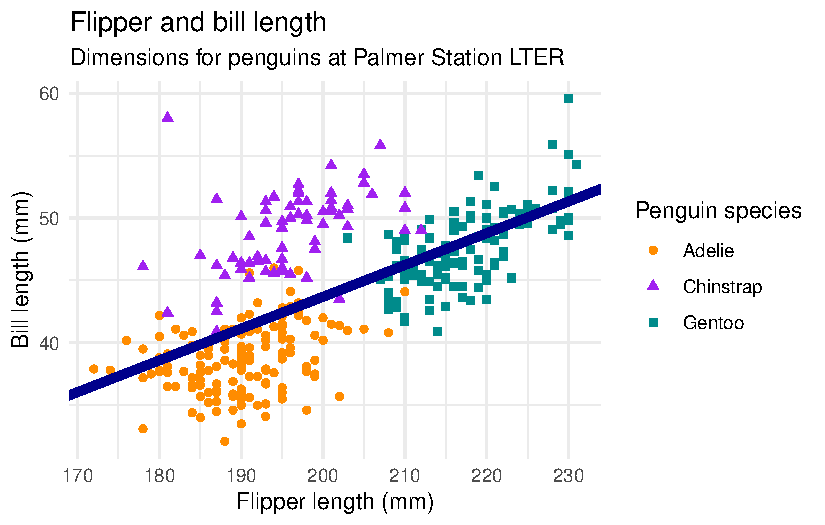
\includegraphics[keepaspectratio]{03-RDATAVIZ_26_quarto_files/figure-pdf/fig-penguins_fit-1.pdf}}

}

\caption{\label{fig-penguins_fit}My first Quarto figure reporting the
fitted line of my first linear model}

\end{figure}%

\subsection{Conclusion}\label{conclusion}

By default, this document is rendered as an HTML file, but Quarto can
generate many other formats as well (check out all the available options
\href{https://quarto.org/docs/output-formats/all-formats.html}{here}).
You can set the default format in the YAML metadata, or generate
multiple formats from the same .qmd file by specifying them in the
terminal, for example:

\begin{Shaded}
\begin{Highlighting}[]
\ExtensionTok{quarto}\NormalTok{ render 03{-}RDATAVIZ\_26\_quarto.qmd }\AttributeTok{{-}{-}to}\NormalTok{ pdf,html}
\end{Highlighting}
\end{Shaded}

The course was designed to teach you state-of-the-art tools for
constructing data storytelling using \texttt{R}. We covered
\texttt{dplyr} for data manipulation, \texttt{ggplot2} for data
visualization, and Quarto as a technical publishing system. Bear in
mind, however, that Data Science is an ever-evolving discipline, and
it's more important than ever to stay updated on active developments.
Specifically, the emerging role of AI is reshaping every phase we've
covered --- from data collection and cleaning to analysis,
visualization, and communication --- and now it's time for a hands-on
session so you can experience these tools in practice!




\end{document}
